% This file was created with tikzplotlib v0.10.1.
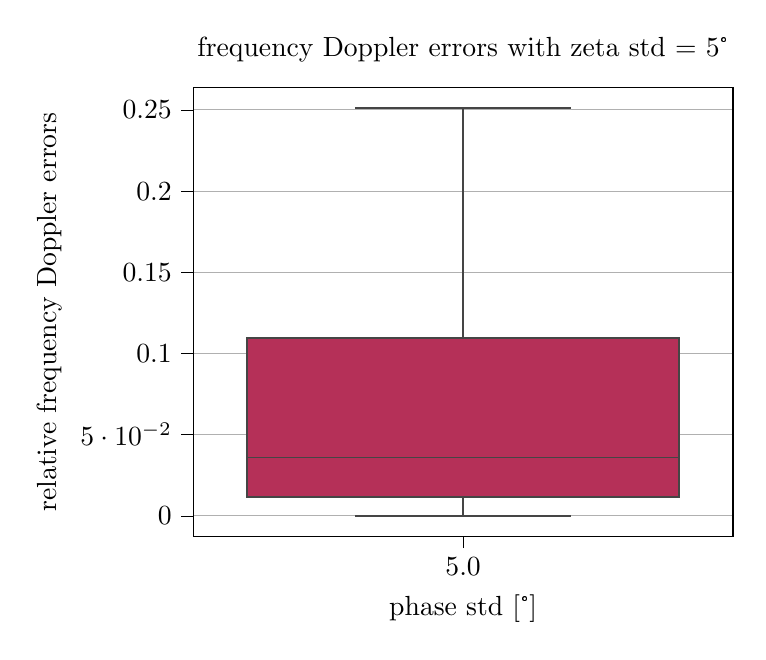
\begin{tikzpicture}

\definecolor{brown1814888}{RGB}{181,48,88}
\definecolor{darkgray176}{RGB}{176,176,176}
\definecolor{darkslategray69}{RGB}{69,69,69}

\begin{axis}[
tick align=outside,
tick pos=left,
title={frequency Doppler errors with zeta std = 5°},
x grid style={darkgray176},
xlabel={phase std [°]},
xmin=-0.5, xmax=0.5,
xtick style={color=black},
xtick={0},
xticklabels={5.0},
y grid style={darkgray176},
ylabel={relative frequency Doppler errors},
ymajorgrids,
ymin=-0.012528815276734, ymax=0.263596085850619,
ytick style={color=black}
]
\path [draw=darkslategray69, fill=brown1814888, semithick]
(axis cs:-0.4,0.0116495818517496)
--(axis cs:0.4,0.0116495818517496)
--(axis cs:0.4,0.10955348528574)
--(axis cs:-0.4,0.10955348528574)
--(axis cs:-0.4,0.0116495818517496)
--cycle;
\addplot [semithick, darkslategray69]
table {%
0 0.0116495818517496
0 2.23165926911539e-05
};
\addplot [semithick, darkslategray69]
table {%
0 0.10955348528574
0 0.251044953981194
};
\addplot [semithick, darkslategray69]
table {%
-0.2 2.23165926911539e-05
0.2 2.23165926911539e-05
};
\addplot [semithick, darkslategray69]
table {%
-0.2 0.251044953981194
0.2 0.251044953981194
};
\addplot [semithick, darkslategray69]
table {%
-0.4 0.0358470601246654
0.4 0.0358470601246654
};
\end{axis}

\end{tikzpicture}
